%% \chapter[htoc-titlei][hhead-titlei]{htitlei}
%% -----------------------------------------------------------------------------
\chapter[Theoretical Background][Theoretical Background]{Theoretical Background}
\label{chapter:theory}
The Standard Model of particle physics (SM) is an extraordinarily successful
description of the fundamental constituents of matter and their interactions.
Many experiments have verified the extremely precise
prediction of the SM. This success has culminated most recently in the
discovery of the Higgs Boson.  This chapter provides a brief introduction to
the structure of the SM and how scientists are able to test it using hadron
colliders. It focuses primarily on the physics of the Higgs boson and its decay
to top quarks.  I stress the importance of a
measurement of the rate at which Higgs Bosons are produced in association of
top quarks, as a new, rigorous test of the SM. The experimental search
for this production mode in multi-lepton final states is the 
general subject of this thesis.


\section{The Standard Model}
\subsection{The Standard Model Structure}

The Standard Model (SM) \cite{np_22_579, prl_19_1264, 1964.Salam-Ward.gauge-theory,1973.Weinberg.SM-with-QCD} is an example of a quantum field theory that describes
the interactions of all of the known fundamental particles. Particles are understood to be excitations of the more fundamental
object of the theory, the field. The dynamics and interactions of the fields are
derived from the Standard Model Lagrangian, which is constructed to be
symmetric under transformations of the group $SU(3) \times SU(2)_L
  \times U(1)$. $SU(3)$ is the group for the color, $SU(2)_L$ is the group 
for weak iso spin, and $U(1)$ is the group for weak hyper-charge.

Demanding these symmetries be local, gauge symmetries allows the theory to be
re-normalizable \cite{1972.tHooft-Veltman.regularization_and_renormalization}, meaning that unwanted infinities can be absorbed into
observables from theory in a way that allows the theory to be able to predict
physics at multiple energy scales.
Gauging the symmetries results in the introduction of 8 massless gluons, or the
boson\footnote{bosons are full integer spin particles that obey Bose-Einstein statistics, while fermions are half-integer spin particles that obey Fermi-Dirac statistics} carriers of the strong force \cite{1973.Gross-Wilczek.Asymptotic_freedom_0} from the generators
$SU(3)$ symmetry, and the 4 massless bosons, carriers for the weak
and electromagnetic forces from the 3 generators of the $SU(2)$ and 1
generator of the $U(1)$ group. The weak and the electromagnetic forces are considered part of a larger single 
unified electroweak group $SU(2) \times U(1)$ and the associated generators mix. 

Matter particles are half-integer spin fermions and are represenations of the symmetry groups. Singlets of the $SU(3)$ 
are called leptons, do not have a color charge, and, therefore, do not interact with the strong force. Quarks,
as triplets of the $SU(3)$ group, do interact with the strong force. The SM is a chiral theory:
the weak force violates parity, as it only couples to left-chiral particles or right-chiral antiparticles. 
This means that right-chiral and left-chiral fermions arise from different fields, which are
different representations of the $SU(2)_L$ group.
 
The discovery of particles and new interactions in various experiments
is intertwined with the development of the theory that spans many
decades and is not discussed in detail here. But these
experiments have proven the above model and symmetries to be an overwhemlimg success.
So far, 3 separate generations of both quarks and leptons have been discovered, differing only by mass. The gluons and the 4 electroweak bosons have also been discovered($W^+$, $W^-$, $Z^0$, and $\gamma$). The reason for this 3-fold replication is not known. Figure~\ref{figure:theory_sm} shows a table of the known SM particle content.  


\begin{figure}[!t]
\centering 
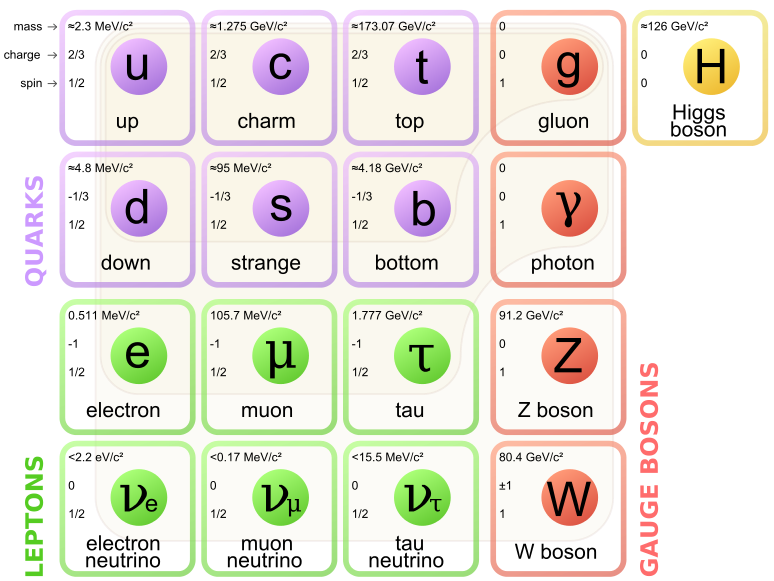
\includegraphics[width=0.9\textwidth]{figs/theory/iaGJO.png}
\caption{ The Standard Model Particle Content
 } \label{figure:theory_sm}
\end{figure}


\subsection{Electroweak Symmetry Breaking and the Higgs}

Despite the simple structure of theory, the discovery of massive fundamental
particles creates two sets of problems both related to $SU(2)_{L} \times U(1)$ symmetry. First, the force-carrying bosons must enter the theory
without mass or the symmetries will be explicitly broken in the Lagrangian. Second, adding
fermion masses to theory in an ad-hoc way allows the right-chiral and
left-chiral fermions to mix. Since they possesses different quantum numbers, as
different representations of the weak-isospin group, this too breaks gauge
invariance. 

To solve these problems, spontaneous electro-weak symmetry breaking (EWSB) is
introduced via the Brout-Englert-Higgs mechanism \cite{Higgs:1964pj, Higgs:1966ev,Englert:1964et}. A  massive scalar field
in an electro-weak doublet is added to the theory with 4 new
degrees of freedom and a potential which includes a 
quartic self-interaction term. Each fermion field interacts with the scalar field via
a different Yukawa coupling, which unites the left and right chiral fields
of a single particle type.  This field
explicitly preserves all of the symmetries, but the minimum of the potential does not
occur when the expectation of the field is zero. The field
eventually falls to a state, where it acquires a non-zero vacuum-expectation
value. A non-vanishing field must point in a
particular direction of weak-isospin space, breaking the symmetry.

The consequences of this spontaneous symmetry breaking are tremendous.
The universe is filled with a field that has a non-zero expectation value.
The theory can be expanded around this new value and 3 of the
degrees of freedom can be interpreted as the longitudinal polarizations of
the $W^+$, $W^-$, and $Z^0$, while the 4th remains a scalar field, called
the Higgs field with an associated particle called the Higgs particle or `Higgs'.
The weak bosons acquire a mass via their longitudinal polarizations and the Yukawa
couplings of the scalar field to the fermions now behave like a mass term
at this new minimum. 


\subsection{The Standard Model Parameters}


Confronting the SM with experiment requires the measurement of
17\footnote{There are additional parameters from neutrino mass terms and
mixing but it is unclear how to include these into the Standard Model,
since it does not predict right-chiral neutrinos} free parameters, which
are unconstrained from the theory. These free parameters include the fermion
masses from the Yukawa couplings, the force coupling constants, the angles and phase of the mixing between
quarks, and constants from the Higgs and electroweak sector\footnote{ The electroweak sector includes
parameters like mass of the $W^{\pm}$ and $Z^0$ bosons, the weak mixing
angle,${\mathrm sin^2}\theta_w$, the fermi constant $G_F$, and Higgs
Mass and vacuum expectation value. These parameters however are not
wholly independent. As discussed above, it is only necessary
theoretically to specify the two parameters relevant to the Higgs
potential and the two coupling associated with the gauge groups }.

%arXiv:1209.2716v2%
Experiments have provided a number of measurements of the
parameters of the SM\cite{lepew:2010vi}.  With the discovery of the Higgs boson and 
the measurement of the Higgs mass, all of the parameters
of the SM can be estimated and statistical procedures can assess
the relative agreement of overlapping measurements to test the self-consistency 
of the SM. The GFitter collaboration assembles
all relevant electroweak observable measurements into a statistical
model and then allows certain measurements to float within their
uncertainty to allow for a fit among multiple correlated measurements\cite{GFitter}. 
These correlations arise for two reasons. First, measurements are made that often
depend on multiple SM parameters. Second, radiative corrections often cause 
parameters to depend on each other. For instance, the Higgs mass is sensitive
to both the $W$ mass and top mass, through loop level corrections. 

Figure \ref{figure:theory_scans} shows the fitted constraints on 4 key SM
parameters ($M_H$, $M_W$, $M_t$, ${\mathrm sin^2}\theta_w$) with
actual measurements overlaid. The plots show both the removal
and inclusion in the fit of key measurements to assess their overall
impact. The addition to the fit of the measured
Higgs mass from the ATLAS and CMS collaborations creates a small
tension, as the other observables prefer the mass to be much
lower ($\sim$ 80 GeV). This tension in the combined
electroweak fit as a result is  not statistically
significant with a $p$-value of 0.07. The
SM seems to be self-consistent. 


\begin{figure}[!t]
\centering 
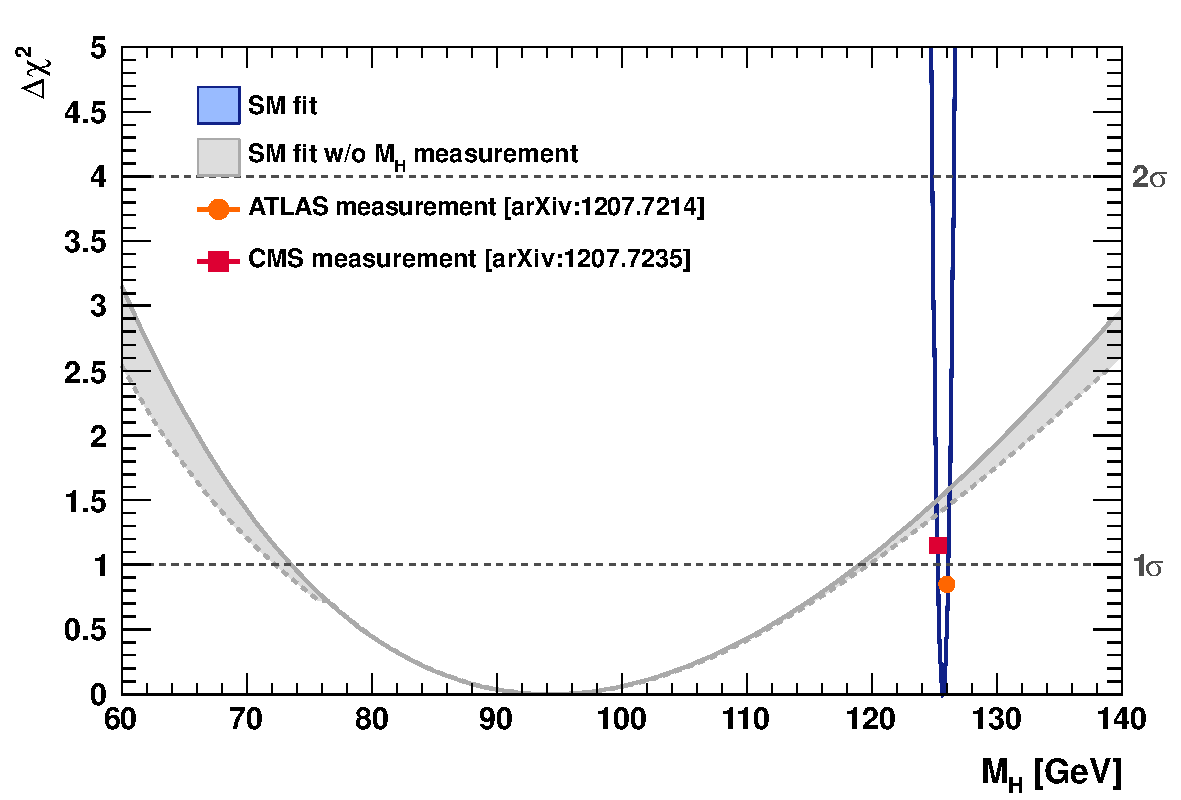
\includegraphics[width=0.45\textwidth]{figs/theory/HiggsScan.pdf}
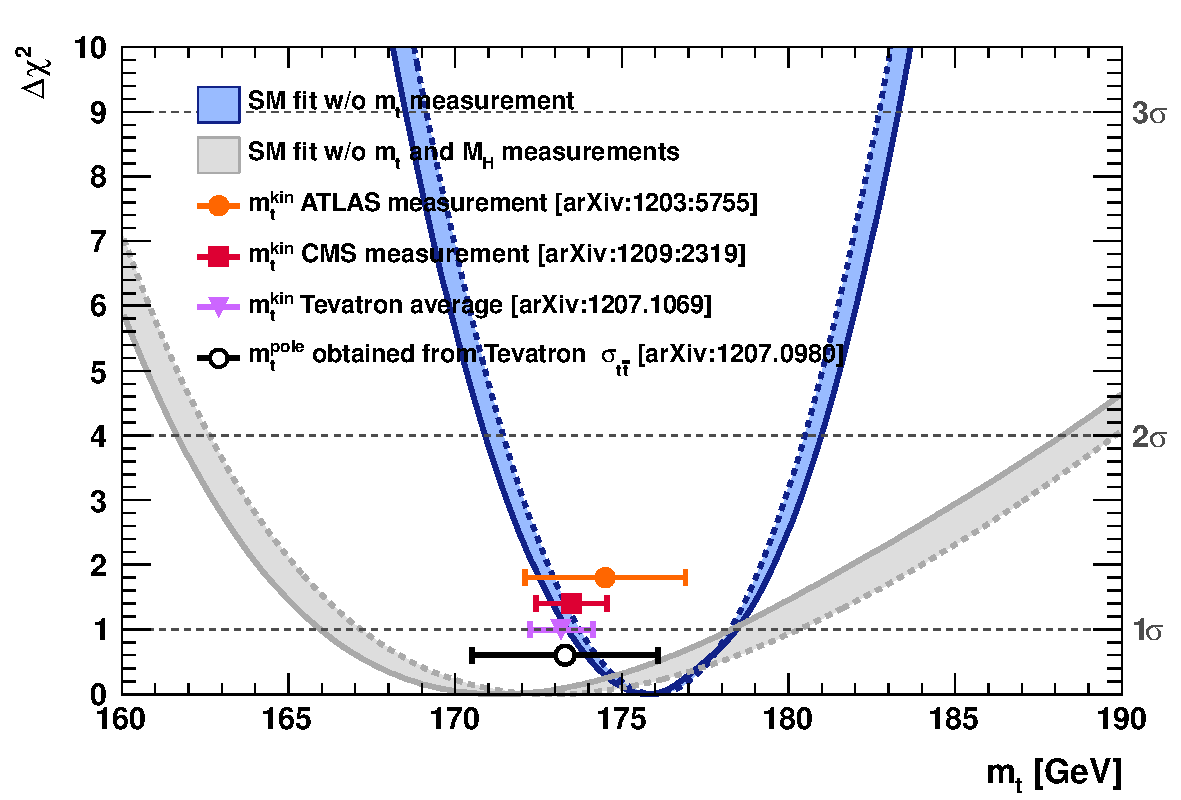
\includegraphics[width=0.45\textwidth]{figs/theory/TopScan.pdf}
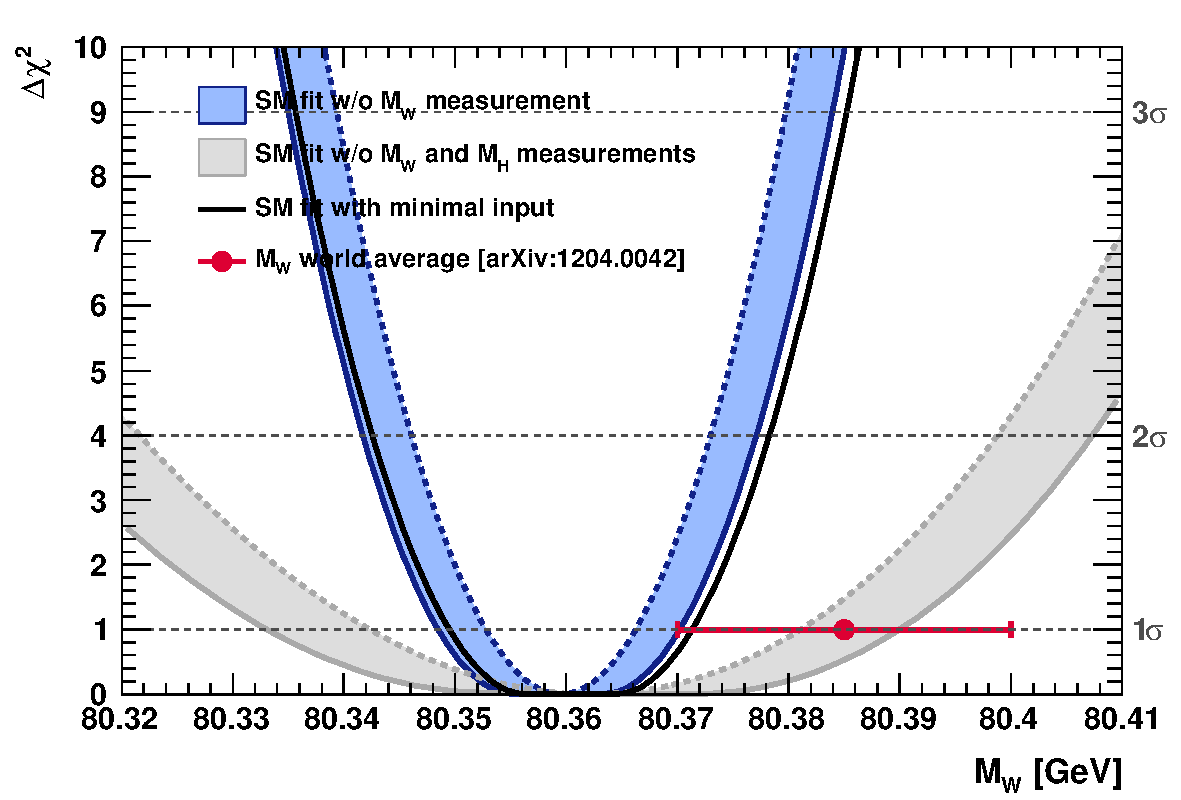
\includegraphics[width=0.45\textwidth]{figs/theory/WMassScan.pdf}
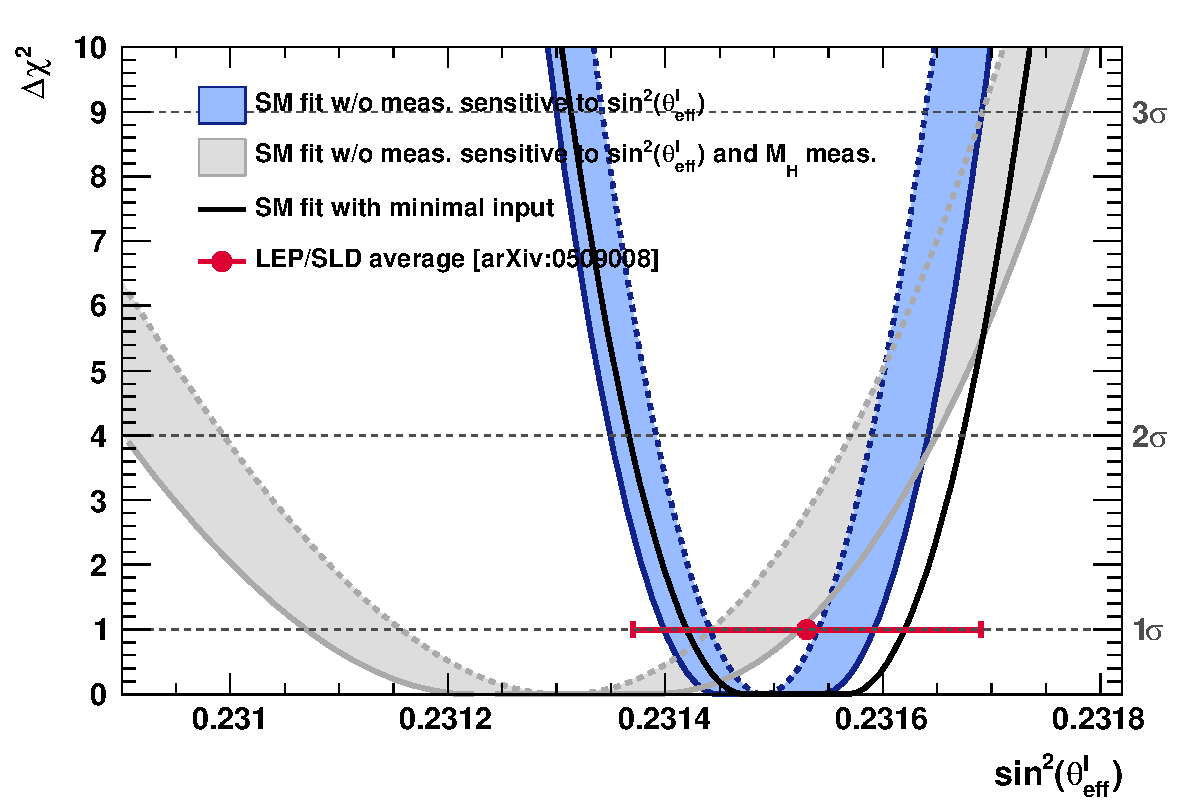
\includegraphics[width=0.45\textwidth]{figs/theory/Sin2ThetaScan.pdf}
\caption{
$\chi^2$ as a function of the Higgs mass (top left), the top quark mass (top
    right), the $W$ boson mass (bottom left) and the effective weak mixing
  angle (bottom right) for the combined SM fit from the GFitter group.  The
  data points placed along $\chi^2=1$ represent direct measurements of the
  respective observable and their $\pm 1\sigma$ uncertainties.  The grey (blue)
  bands show the results when excluding (including) the new $M_H$ measurements
  from (in) the fits. } \label{figure:theory_scans}
\end{figure}


\section{Collider Physics and the Higgs} 

To test the theory, physicists accelerate particles to extremely high energies and force
them to interact through collisions. Typically, the particles accelerated are
electrons or protons, since they are stable. Electron-positron collider
machines have a rich history of discovery and measurement in particle physics.
The advantage of electron accelerators is that the colliding element is itself
a fundamental particle. However, due to synchrotron radiation, the curvature of the
beam line becomes problematic for high energy beams.  On the other
hand, proton-proton and proton-anti-proton colliders can be accelerated in rings without large losses
due to synchrotron radiation, but the actual colliding objects at high
energies are the constituent quarks and gluons. This complicates analysis
because the initial state of the hard-scattering system is not known on a per-collision
basis and the momentum of hard-scattering system is unknown along the beam direction.

For hadron colliders, physicists must rely on form-factor descriptions of the colliding hadrons
that describe the fraction of momentum carried by the
hadrons constituent `partons'.  These are called parton distribution
functionsi (PDF), seen in Figure \ref{figure:theory_pdf}, and are factorized
and integrated through the theoretical calculations of various collision processes \cite{1985.Collins.factorization-theorem}.

%http://arxiv.org/pdf/0901.0002v3.pdf
At the Large Hadron Collider (LHC) protons are collided.The types of initial hard-scattering states at the LHC are quark-quark, quark-gluon, and gluon-gluon. Gluon collisions dominate overall,
  due to the large number of gluons inside the proton, though the relative importance of different initial states changes with the
  energy scale of the collision and the type of final state selected.  

\begin{figure}[!t]
\centering 
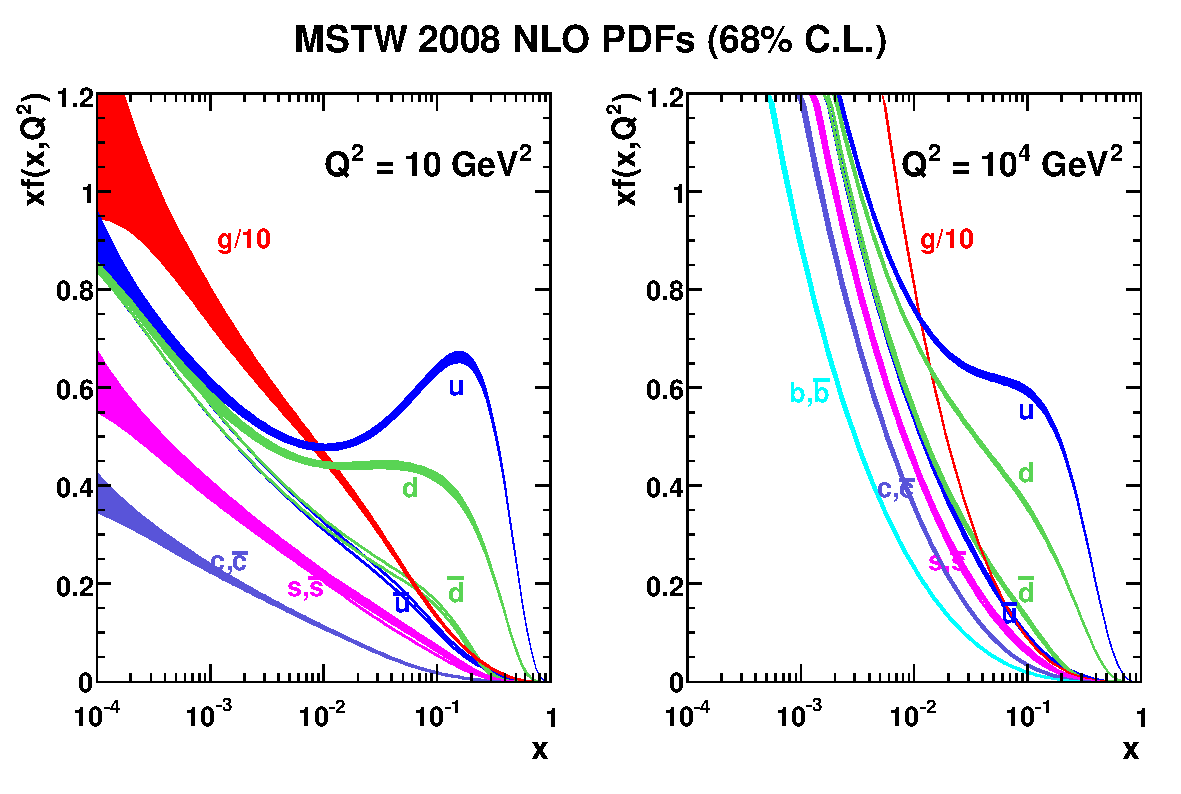
\includegraphics[width=0.8\textwidth]{figs/theory/mstw2008nlo68cl_allpdfs.pdf}
\caption {Proton Parton Distribution Functions (PDFs) from the MSTW Collaboration at $Q^2 = 10$ GeV$^2$ and $Q^2 = 10^4$ GeV$^2$}.
\label{figure:theory_pdf}
\end{figure}

%
A prime motivation for the construction of the Large Hadron Collider was the
discovery or exclusion of the Higgs boson\cite{lhcProposal}. LEP and the Tevatron excluded large
swaths of possible Higgs boson masses, especially below 114 GeV. The Higgs mass was also known to 
have a theoretically motivated upper bound. The unitarity of diagrams including the $WWWW$ vertex required the Higgs mass to
be below about 1 TeV. The LHC was designed to be able to eventually find or exclude 
a Higgs particle in this range \cite{lepew:2010vi}. 

Reaching this discovery or exclusion required an enormous
dataset with collisions at high energies. Despite the fact that the Higgs couples to nearly
every particle, Higgs boson production at the LHC is a
low rate process. Because it couples to fermions proportional to mass and
because the colliding particles must be stable and therefore light, production
of the Higgs must occur through virtual states. 

\begin{figure}[!t]
\centering
\begin{tabular}{cc}
\subfloat[ggF]{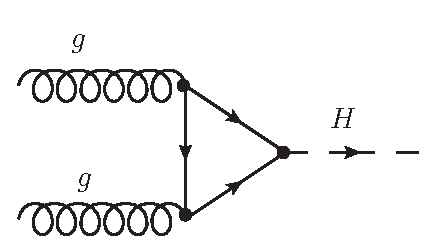
\includegraphics[width=0.35\textwidth]{figs/theory/ggF.pdf}} &
\subfloat[VBF]{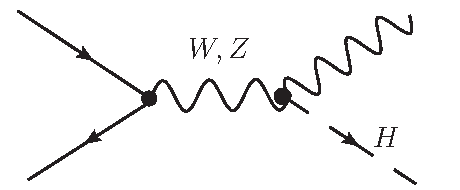
\includegraphics[width=0.35\textwidth]{figs/theory/vh.pdf}} \\
\subfloat[VH]{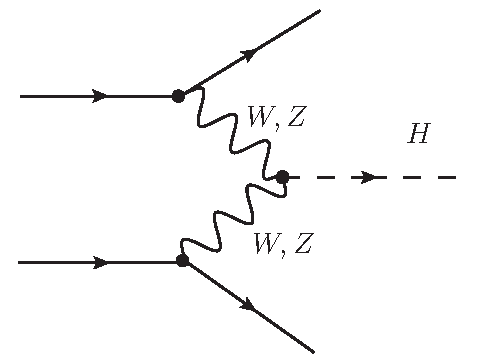
\includegraphics[width=0.35\textwidth]{figs/theory/vbf.pdf}} &
\subfloat[$t\bar{t}H$]{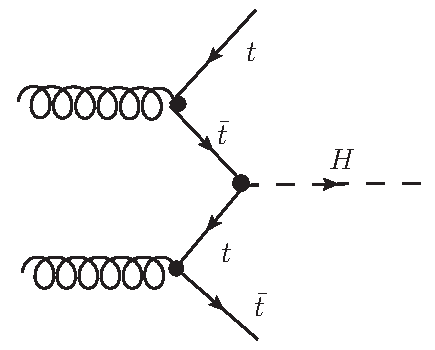
\includegraphics[width=0.35\textwidth]{figs/theory/tth.pdf}} \\
\end{tabular} 
\caption{Dominant Higgs production modes at the LHC}
\label{figure:theory_higgsdiagrams}
\end{figure}


The Higgs boson can be produced through collision at the LHC
via 4 mechanisms: gluon-fusion (ggF), vector-boson fusion (VBF), 
Higgsstrahlung (VH), and production in association with top quarks ($t\bar{t}H$). The diagrams
are shown in Figure \ref{figure:theory_higgsdiagrams} and the production
cross-sections as a function of Higgs mass for the 8 TeV LHC proton-proton
running are shown in Figure \ref{figure:theory_xsec} \cite{Dittmaier:2012vm}. The largest production
cross-section is via the gluon fusion channel at ~$20$ pb, which proceeds
through a fermion loop that is dominated by the top quark, because of its
large Yukawa coupling to the Higgs. Because the Higgs couples to every massive
particle, it has a rich set of decays also seen in Figure
\ref{figure:theory_xsec}, especially for $m_H=125$ GeV.  Studies of Higgs
properties at hadron colliders offers many tests of the Standard Model
and ample room for new physics searches. These
tests specifically can verify the link between Yukawa coupling and the
particles mass and further constrain details of EWSB by examining Higgs coupling
to the weak bosons. 

\begin{figure}[!t]
\centering 
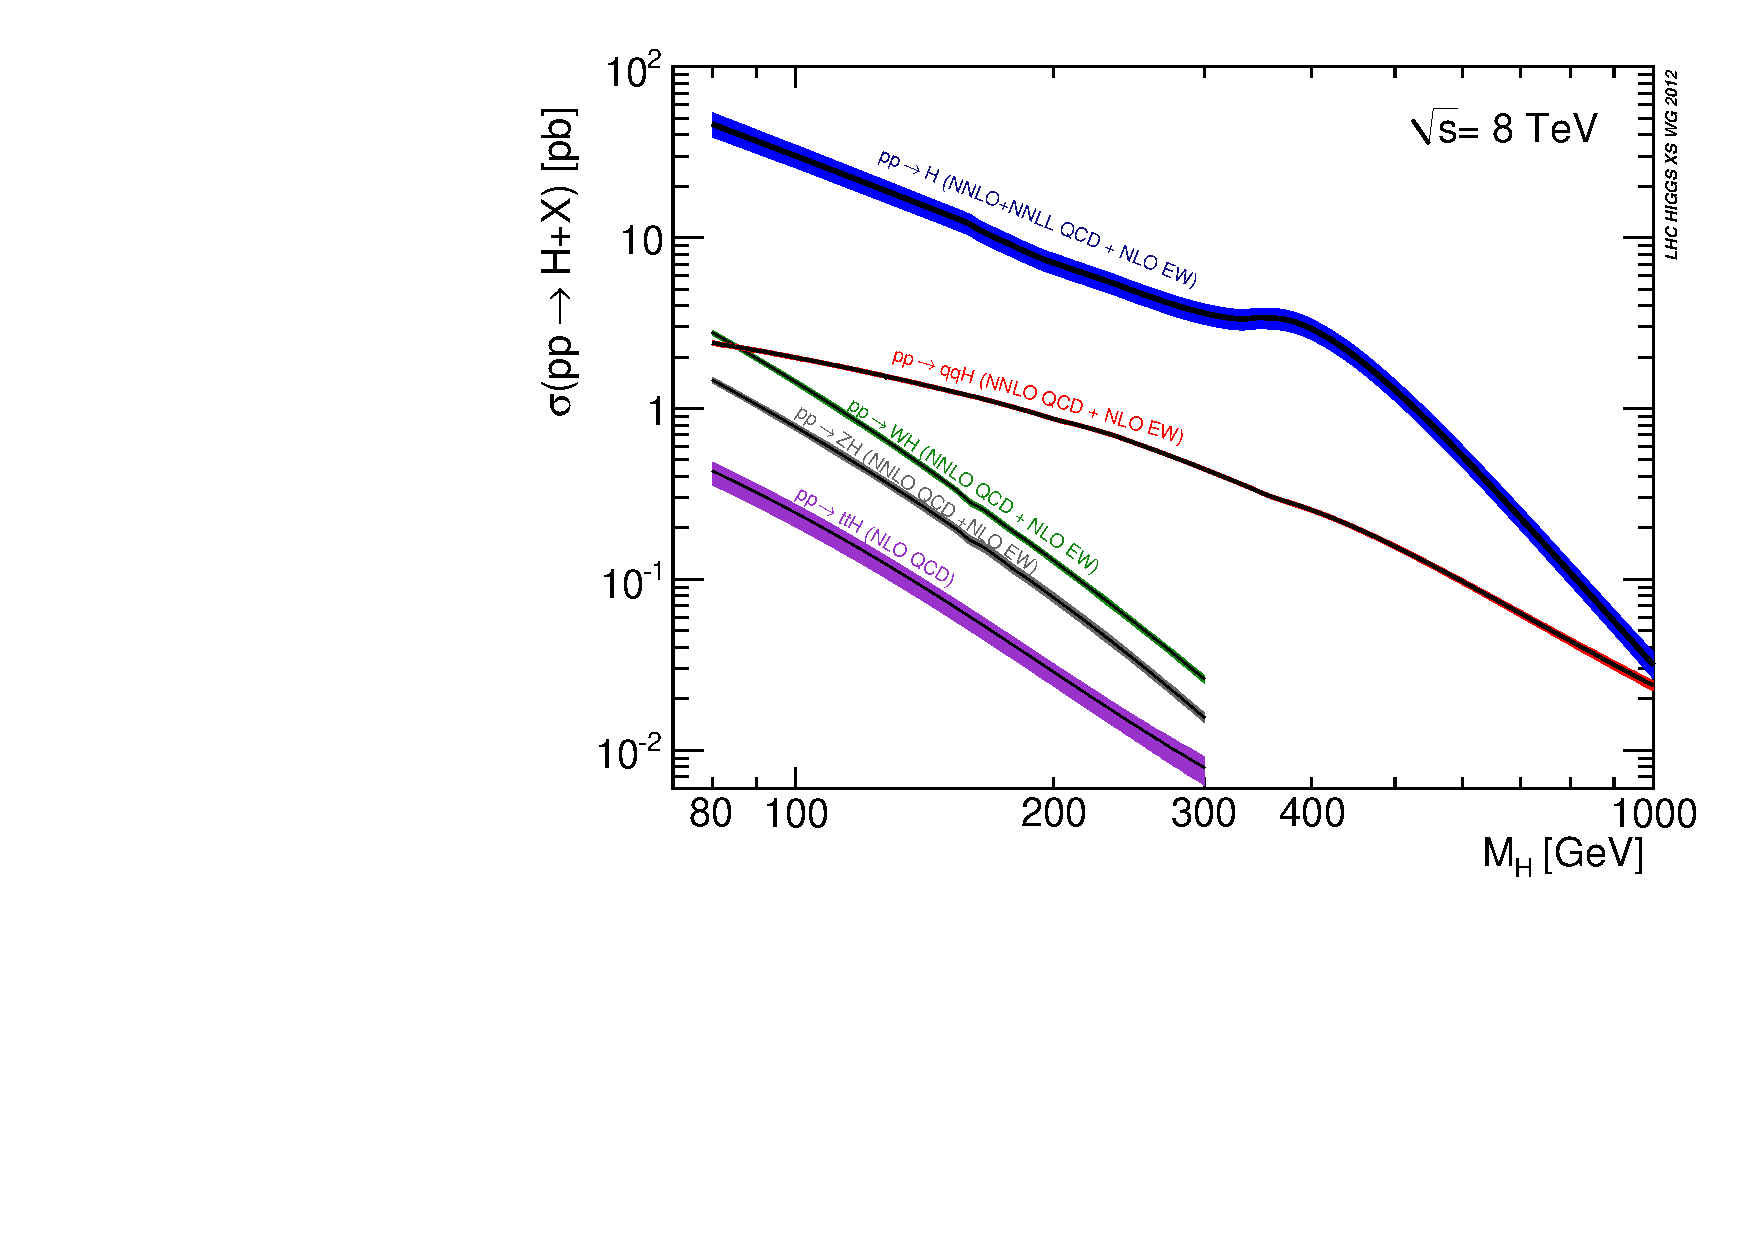
\includegraphics[width=0.52\textwidth]{figs/theory/Higgs_XS_8TeV_lx.pdf}
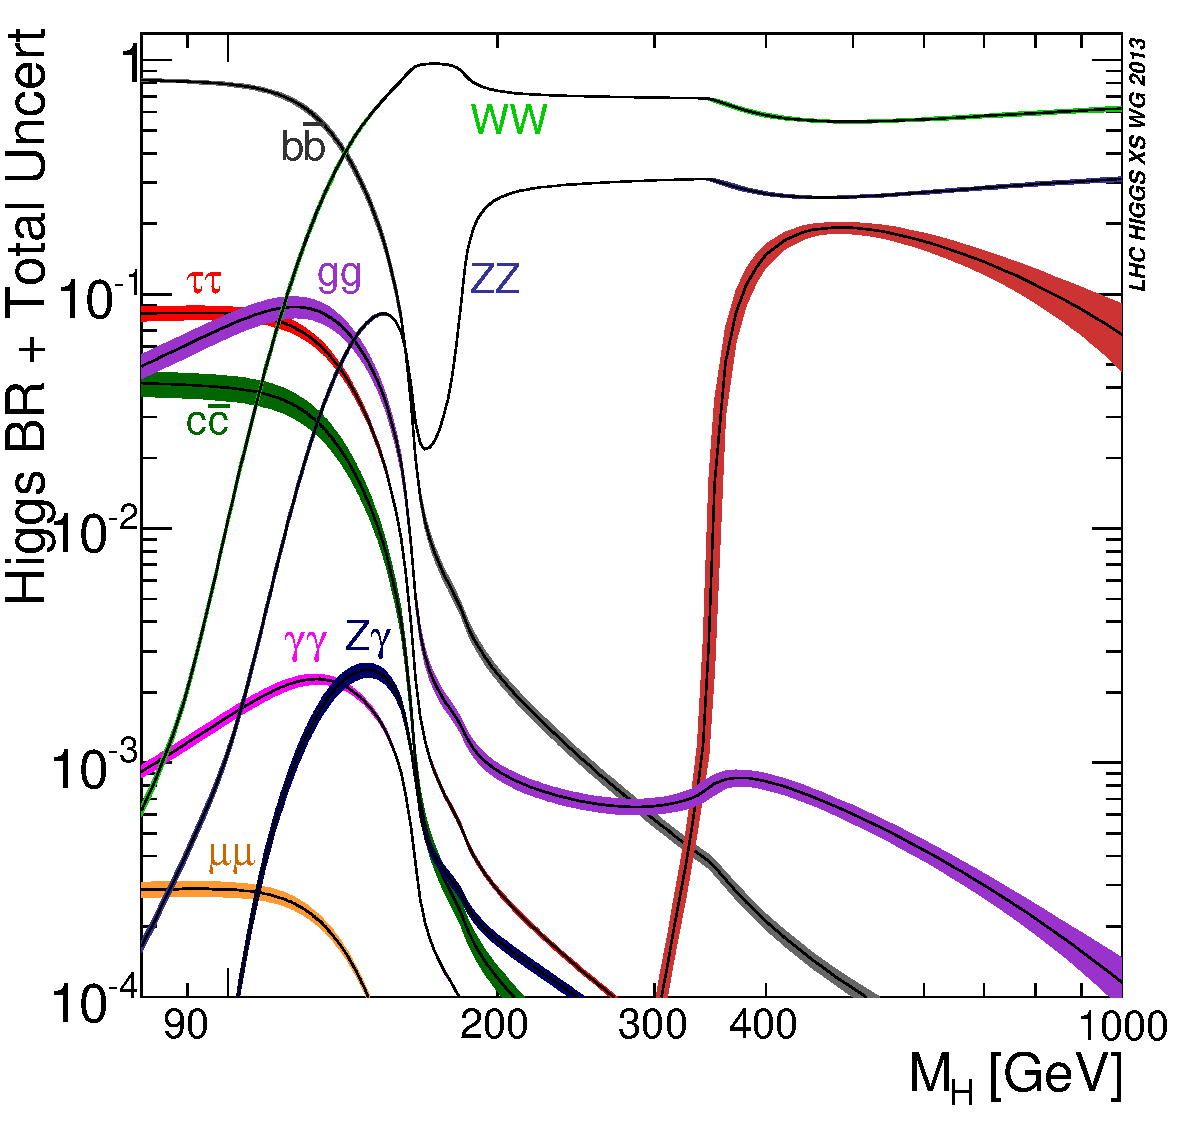
\includegraphics[width=0.42\textwidth]{figs/theory/Higgs_BR.pdf}
\caption {8 TeV LHC Higgs production cross-sections (left) and decay branching fractions }.
\label{figure:theory_xsec}
\end{figure}


\subsection{Higgs Discovery at the LHC}

In 2012 both ATLAS and CMS announced the discovery of a new boson consistent
with the Higgs by examining the results of Higgs searches in a number of decay
channels ($H\rightarrow W^+W^-$,$H\rightarrow Z^0Z^0$, and
    $H\rightarrow\gamma\gamma$) in the 2011 dataset at $\sqrt{s}=$7 TeV and
part of the 2012 dataset at $\sqrt{s}=$8 TeV. By 2013 and 2014, both
experiments have updated and/or finalized their results for the full 2011 and
2012 datasets \cite{ATLAS-CONF-2014-009,CMS-PAS-HIG-14-009}. I will focus on the ATLAS results, 
which measured both the Higgs mass\cite{Aad:2014aba} and spin\cite{tagkey2013120}, as well as 
provided initial constraints of the Higgs couplings to different particles. 

Figure \ref{figure:theory_higgsdisc} show the results of the searches in all of the
measurement channels as well as constraints on the SM Higgs coupling parameters in 
an example fit, where the couplings to the top-quark, bottom-quark, W,Z, and $\tau$
are allowed to fluctuate independently. These rely on measurements binned in different
production and decay channels. They are dominated by higher statistics results in the 
gluon-fusion production modes, but measurements in the VH and VBF modes are close to 
SM sensitivity. 

The combined results show basic agreement with the SM with much room for improvement
with the addition of new production and decay modes and higher statistics. The 
coupling constraints are particularly strong for the W and Z, which are
the most sensitive decay channels, and top quark due to the dominance of the
top Yukawa in the ggF loop. 


\begin{figure}[!t]
\centering 
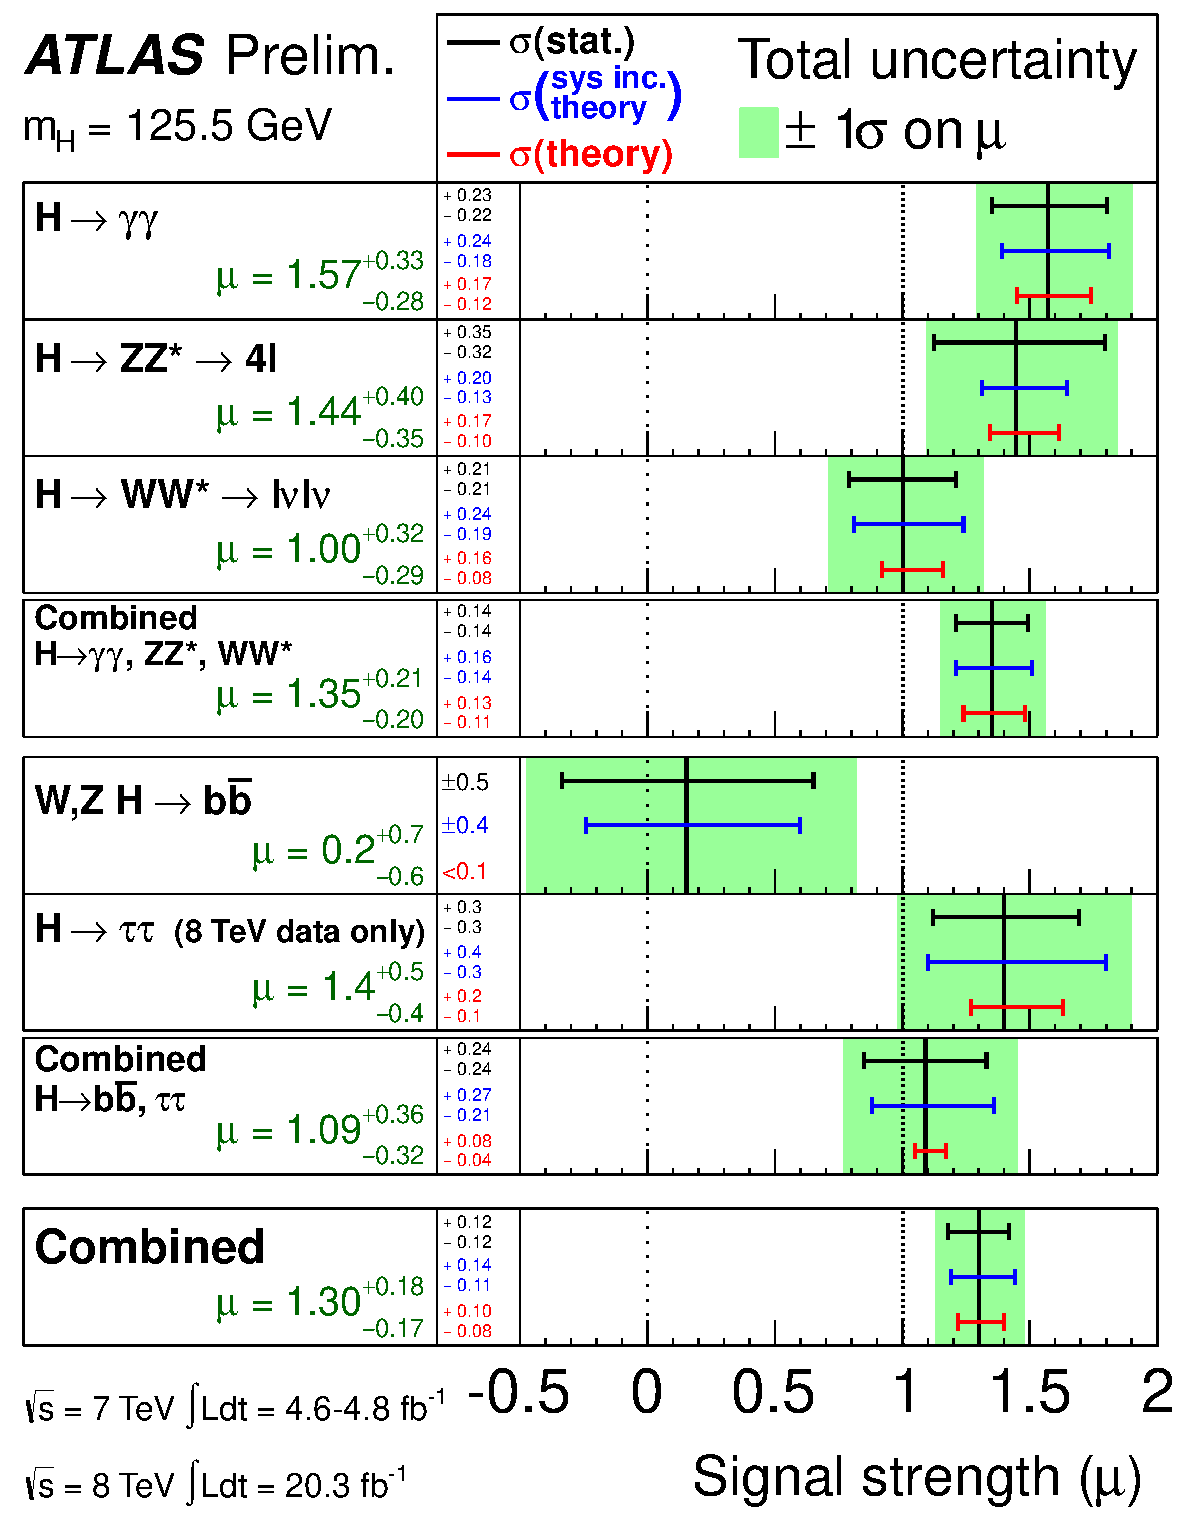
\includegraphics[width=0.45\textwidth]{figs/theory/atlas_higgs.pdf}
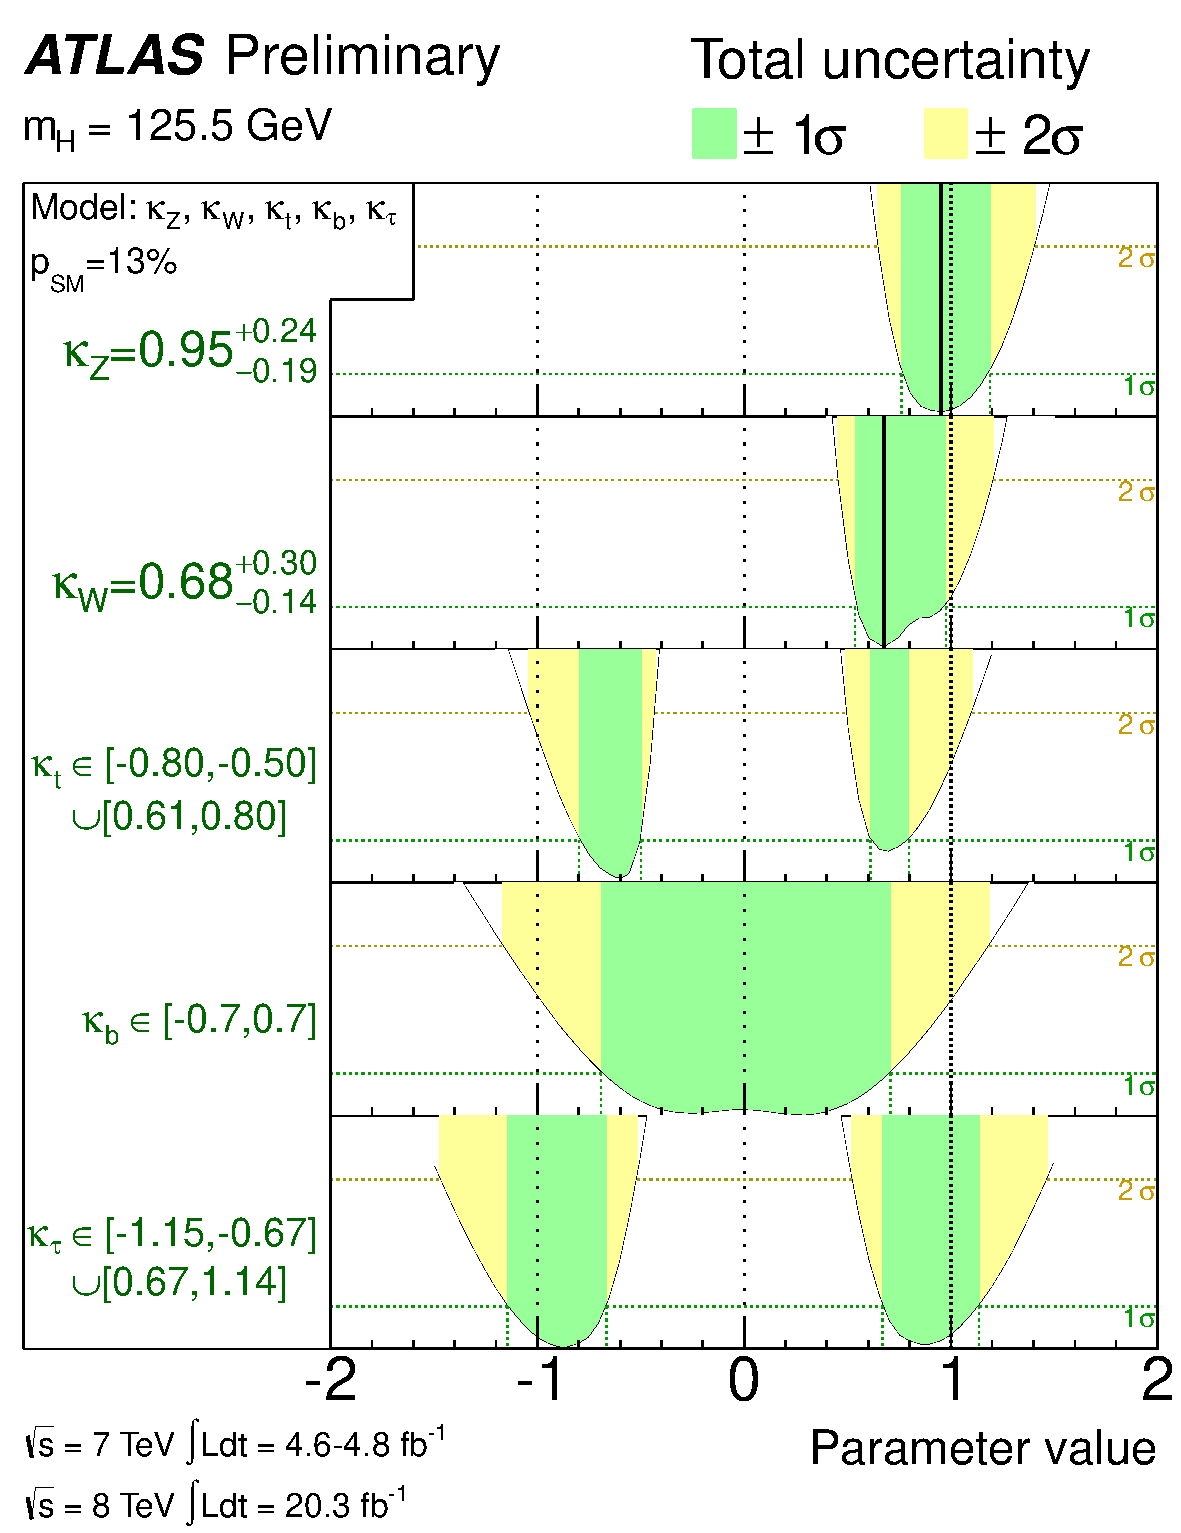
\includegraphics[width=0.45\textwidth]{figs/theory/atlas_coupling.pdf}
\caption {
  ATLAS Higgs combination results for all SM measurement channels as ratios of
  the measured to SM production cross-sections (left) and extracted Higgs
  coupling constraint scale-factors for a combined fit to the measurement
  channels, where the W,Z, top-quark, b-quark, and $\tau$ couplings are
  allowed to float. The p-value of this particular model is 0.13 and in agreement
  with SM expectations}

\label{figure:theory_higgsdisc}
\end{figure}


\subsection{The Importance $t\bar{t}H$ Production}

Notably absent thus far in the SM are searches for the Higgs in the $t\bar{t}H$
production channel, due to the low production rate and lack of statistics. Searches are underway and
initial results are close to SM sensitivity for ATLAS and CMS.

Measuring the $t\bar{t}H$ production rate is important, because
$t\bar{t}H$ production depends on the top Yukawa coupling at tree level. Comparing
the predicted Yukawa coupling from top mass measurements to the coupling from
the wholly independent Higgs production measurements is a very direct 
test of the Higgs' involvement in providing mass for the fermions in the SM.

The top Yukawa coupling is already constrained from current measurements of the ggF production
process, since the ggF loop is dominated by top quarks. However, new, colored particles could be
present in the loop. Comparison of the gluon-fusion and the $t\bar{t}H$
modes would allow for disentangling the effects of these possible new particles\cite{Dawson:2013bba}. 
The simplest of new phyiscs models, allowing for the modification
of the ggF loop, introduce a new generation of quarks. However, fourth
generation quarks, which obtain mass from a Higgs Yukawa coupling, are already
largely excluded due to their enormous effects on the Higgs production
cross-section\cite{Eberhardt:2012gv}. Other exotic scenarios allow for new colored particles, 
which are not entirely constrained by present measurements\cite{Carena:2013iba,ArkaniHamed:2012kq,Carmi:2012yp}.
These include, for instance, supersymmetric models involving the stop quark.  

With the level of statistics available in Run I dataset, very strict constraints on the top 
Yukawa coupling are simply not possible and the measurment presented in this 
thesis is a first step. Future, high-statistics datasets will have the ability to provide 
better measurements and \tth\ production will become very important.
Despite similar uncertainties on the overall production cross-sections for $t\bar{t}H$ and the ggF,
\tth\ has the advantage that most of these uncertainties would cancel for $t\bar{t}H$ if normalized to the topologically similar $t\bar{t}Z$.  Finally, the uniqueness of the experimental signature means that
searches for $t\bar{t}$ signatures can be performed for a variety of Higgs decays ($\gamma\gamma$, $b\bar{b}$,
$WW$,$ZZ$, and $\tau\bar{\tau}$ with roughly similar degrees of sensitivity (within a factor of 10)\cite{Dawson:2013bba}. 


It is important to note the importance of the top Yukawa coupling
due to its enormous size compared to other couplings. For instance, the top Yukawa is 350000x as large as the electron
Yukawa coupling. The top Yukawa coupling,
along with the Higgs mass, is one of the most important pieces of the renormalization group equations (RGE)
responsible for the running of the parameter that determines the Higgs self-coupling $\lambda$. 
If this parameter runs negative, then the potential responsible for the entire mechanism 
of EWSB no longer has a minimum and becomes unbounded, resulting in instability in the universe \cite{Degrassi:2012ry}.
Metastability occurs when the shape of the potential allows for a false local minimum.
Figure \ref{figure:theory_stability} shows the running of this parameter, the regions
for which the universe is stable, unstable and metastable. Current
measurements suggest that universe lies in a metastable island\footnote{The
RGE assumed that there is no new physics at all energy scales}. This is a sort of fanciful
aside, intended only to highlight the importance of the top Yukawa coupling and to suggest that
new discoveries in the top-Higgs sector have far reaching consequences. 


\begin{figure}[!t]
\centering 
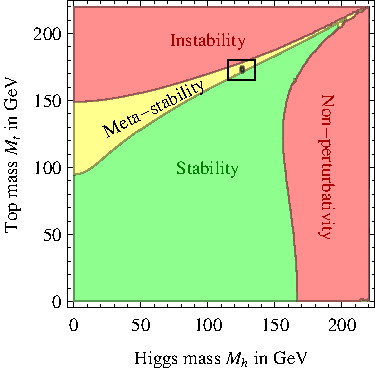
\includegraphics[width=0.45\textwidth]{figs/theory/SMstability.pdf}
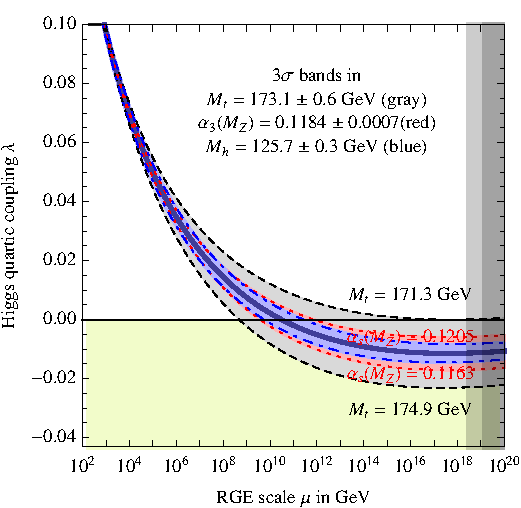
\includegraphics[width=0.45\textwidth]{figs/theory/runLambda.pdf}
\caption {
  RGE for the running of the SM parameter, $\lambda$ for the Higgs self-coupling term 
  with present values and uncertainty bands for $M_H$ and $M_t$ (left). The two-dimensional
  plot colored (right) shows regions for which the SM is stable, unstable and metastable
  based on this RGE.}

\label{figure:theory_stability}

\end{figure}


\section{Conclusion}

The Standard Model, despite its success in providing a unified description of fundamental
particles and interactions into single theory, has its flaws. These have been discussed in 
depth elsewhere, but include issues like the description of massive neutrinos, the failure
to include gravity, and the unnaturalness of large quantum corrections to Higgs parameters.
For these reasons, it seems the SM might be a lower energy approximation to a more fundamental
theory. The discovery of the Higgs boson at the LHC provided a stunning verification of one
of the fundamental aspects of the theory but at the same time offers new area to search for
glimpses of something more fundamental. The production of samples of Higgs bosons
allows for a rich array of new tests of the Standard Model, which is now finally over-constrained by experiment. 
Searches for the $t\bar{t}H$ production, one category of which is the topic
of this thesis, provide tree-level access to a central parameter of the theory, the top Yukawa coupling,
as well as access a variety of Higgs decays, which will eventually provide a rigorous new 
test of the SM. 


